%% LyX 2.3.6.1 created this file.  For more info, see http://www.lyx.org/.
%% Do not edit unless you really know what you are doing.
\documentclass[english]{article}
\usepackage[T1]{fontenc}
\usepackage[latin9]{inputenc}
\usepackage{float}
\usepackage{url}
\usepackage{amsmath}
\usepackage{amssymb}
\usepackage{graphicx}

\makeatletter

%%%%%%%%%%%%%%%%%%%%%%%%%%%%%% LyX specific LaTeX commands.
%% Because html converters don't know tabularnewline
\providecommand{\tabularnewline}{\\}
\floatstyle{ruled}
\newfloat{algorithm}{tbp}{loa}
\providecommand{\algorithmname}{Algorithm}
\floatname{algorithm}{\protect\algorithmname}

\makeatother

\usepackage{babel}
\begin{document}
\title{Locate the parameters of RBF networks using a hybrid Particle Swarm
Optimization method}
\author{Ioannis G. Tsoulos, Vasilieos Charilogis}
\date{Department of Informatics and Telecommunications, University of Ioannina,
Greece}
\maketitle
\begin{abstract}
The present paper proposes a two-phase technique for training RBF
neural networks. In the first phase, a hybrid algorithm combining
interval techniques and particle swarm optimization is used to detect
the initialization interval of the neural network parameters. In the
second phase, a hybrid algorithm that conjuncts particle swarm optimization
and local minimization is used to train the neural network within
the space identified in the first phase. This technique is evaluated
on a number of regression and classification datasets from the relevant
literature.
\end{abstract}

\section{Introduction }

Regression and data classification are two major categories of problems
that are solved with machine learning techniques. Such problems appear
regularly in scientific areas such as physics \cite{physics_ml1,physics_ml2},
chemistry \cite{chemistry_ml1,chemistry_ml2}, economics \cite{econ_ml1,econ_ml2},
medicine \cite{med_ml1,med_ml2}, etc. A programming tool that is
used quite often to handle such problems is the RBF artificial neural
network \cite{rbf1}. An RBF networks can be expressed as a function:\textbf{
\begin{equation}
y\left(\overrightarrow{x}\right)=\sum_{i=1}^{k}w_{i}\phi\left(\left\Vert \overrightarrow{x}-\overrightarrow{c_{i}}\right\Vert \right)\label{eq:firstrbf}
\end{equation}
}The following applies to the above equation
\begin{enumerate}
\item The vector $\overrightarrow{x}$ is the input pattern to the equation.
The number of values in this vector is denoted as $d$.
\item The vectors $\overrightarrow{c_{i}},\ i=1,..,k$ are denoted as the
center vectors.
\item The vector $\overrightarrow{w}$ is considered as the output weight
of the RBF network.
\item The value $y\left(\overrightarrow{x}\right)$ is the predicted value
of the network for the pattern $\overrightarrow{x}$.
\end{enumerate}
Typically, the function $\phi(x)$ is a Gaussian function defined
as:\textbf{
\begin{equation}
\phi(x)=\exp\left(-\frac{\left(x-c\right)^{2}}{\sigma^{2}}\right)
\end{equation}
}A plot for the Gaussian function with $c=0,\ \sigma=1$ is shown
in Figure \ref{fig:gauss}. As can be seen from the figure, the value
of the function decreases as we move away from the center. An extensive
overview of RBF networks is given in the work of Ghosh and Nag \cite{rbfghosh}.
RBF networks are used as approximation tools in various cases, such
as  solutions of differential equations \cite{rbfde1,rbfde2},\textbf{
}digital communications \cite{rbfnetwork1,rbfnetwork2},\textbf{ }physics
\cite{rbfphysics1,rbfphysics2}, chemistry \cite{rbfchemistry1,rbfchemistry2},\textbf{
}economics \cite{rbfecon0,rbfecon1,rbfecon2}, network security \cite{rbf_dos1,rbf_dos2}
etc. RBF networks are thoroughly discussed in\textbf{ }\cite{rbfadv}
and it has been parallelized in a variety of research papers \cite{rbfpar1,rbfpar2}.
This model has been extended by various researchers in tasks such
as creating new initialization techniques for the network parameters,\textbf{
}\cite{rbfinit1,rbfinit2,rbfinit3}, pruning techniques\textbf{ }\cite{rbfprun1,rbfprun2,rbfprun3},
construction of RBF networks \cite{rbfcon1,rbfcon2,rbfcon3} etc.
In the current work, a hybrid technique is proposed for the optimal
calculation of the parameters of an RBF network. This technique consists
of two phases: during the first phase a range of values for the network
parameters is estimated using an interval technique, guided by a Particle
Swarm Optimizer (PSO). In the second phase, the network parameters
are optimized within the optimal value interval of the first phase
using a genetic algorithm.

The rest of this article is organized as follows: in section \ref{sec:Method-description}
the two phases of the proposed method are thoroughly discussed, in
section \ref{sec:Experiments} the experimental datasets are listed
as well as the experimental results and finally in section \ref{sec:Conclusions}
some conclusions are presented.

\begin{figure}
\caption{Typical plot for the Gaussian function.\label{fig:gauss}}

\centering{}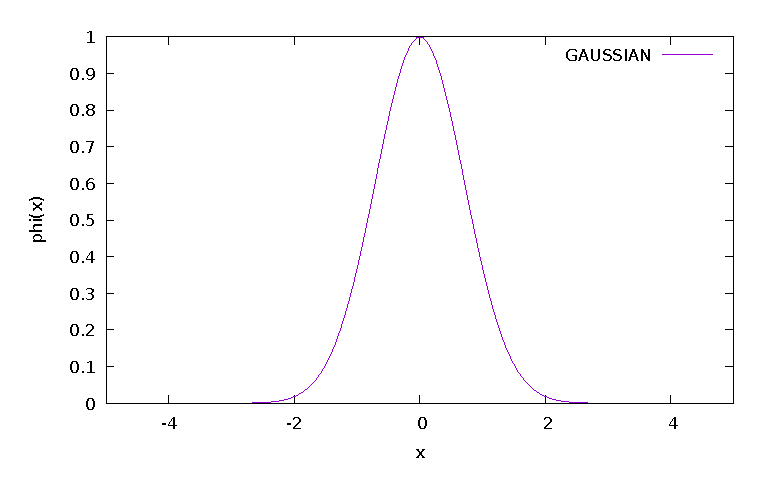
\includegraphics{gaussian}
\end{figure}


\section{Method description \label{sec:Method-description}}

The training error of the RBF network is expressed as: 
\begin{equation}
E(y(x,g))=\sum_{i=1}^{m}\left(y\left(x_{i},g\right)-t_{i}\right)^{2}\label{eq:eqrbf}
\end{equation}
where $m$ is the number of patterns and $t_{i}$ is the output for
pattern $x_{i}$. The vector $g$ is the set of the parameters of
the RBF network. Usually, RBF networks are trained through a two phase
procedure: 
\begin{enumerate}
\item In the first phase the $k$ centers as well as the associated variances
are estimated through K-Means algorithm \cite{kmeans}. A typical
formulation of the K-Means algorithm is outlined in Algorithm \ref{alg:The-K-Means-algorithm.}.
\item In the second phase, the weight vector $\overrightarrow{w}=\left(w_{1},w_{2},\ldots,w_{k}\right)$
is estimated by solving a linear system of equations.
\begin{enumerate}
\item \textbf{Set} \textbf{$W=w_{kj}$}
\item \textbf{Set} \textbf{$\Phi=\phi_{j}\left(x_{i}\right)$}
\item \textbf{Set $T=\left\{ t_{i}=f\left(x_{i}\right),i=1,..,M\right\} $. }
\item The system to be solved is identified as:\textbf{ 
\begin{equation}
\Phi^{T}\left(T-\Phi W^{T}\right)=0
\end{equation}
}With solution:\textbf{
\begin{equation}
W^{T}=\left(\Phi^{T}\Phi\right)^{-1}\Phi^{T}T=\Phi^{\dagger}T\label{eq:eqoutput}
\end{equation}
}
\end{enumerate}
\end{enumerate}
The proposed work uses two computational phases to optimally calculate
the network parameters. In the first phase, a promising range for
the parameters of the network is calculated through an optimization
process that incorporates interval arithmetic. In the second phase,
the parameters of the network are trained with the usage of a genetic
algorithm inside the located range of the first phase. The following
subsections analyze both of these phases in detail.

\begin{algorithm}
\caption{The K-Means algorithm.\label{alg:The-K-Means-algorithm.}}

\begin{enumerate}
\item \textbf{Repeat}
\begin{enumerate}
\item $S_{j}=\left\{ \right\} ,\ j=1..k$
\item \textbf{For} each sample $x_{i},\ i=1,...,m$ \textbf{Do}
\begin{enumerate}
\item \textbf{Calculate} $j^{*}=\min_{i=1}^{k}\left\{ D\left(x_{i},c_{j}\right)\right\} $,
the nearest center for sample $x_{i}$.
\item \textbf{Set} $S_{j^{*}}=S_{j^{*}}\cup\left\{ x_{i}\right\} $.
\end{enumerate}
\item \textbf{EndFor}
\item \textbf{For} every center $c_{j},\ j=1..k$ \textbf{Do}
\begin{enumerate}
\item \textbf{Define} $M_{j}$ as the number of elements in $S_{j}$
\item \textbf{Calculate }$c_{j}$
\[
c_{j}=\frac{1}{M_{j}}\sum_{i=1}^{M_{j}}x_{i}
\]
\end{enumerate}
\item \textbf{EndFor}
\end{enumerate}
\item \textbf{Calculate} the variances for every center as 
\[
s_{j}^{2}=\frac{\sum_{i=1}^{M_{j}}\left(x_{i}-c_{j}\right)^{2}}{M_{j}}
\]
\item \textbf{Terminate }if there is no change in centers $c_{j}$.
\end{enumerate}
\end{algorithm}


\subsection{Preliminaries }

In order to perform interval arithmetic on RBF networks the following
definitions are introduced:
\begin{enumerate}
\item The comparison of two intervals $W=\left[w_{1},w_{2}\right]$, $Z=\left[z_{1},z_{2}\right]$
is performed through the function 
\begin{eqnarray}
L^{*}(W,Z) & = & \begin{cases}
\mbox{TRUE}, & w_{1}<z_{1},\mbox{OR\ \ensuremath{\left(w_{1}=z_{1}\ \mbox{AND}\ w_{2}<z_{2}\right)}}\\
\mbox{FALSE}, & \mbox{\mbox{OTHERWISE}}
\end{cases}\label{eq:eql}
\end{eqnarray}
\item The function $E(y)$ (equation \ref{eq:eqrbf}) is modified to an
interval one
\begin{equation}
[E_{min},E_{max}]=\sum_{i=1}^{M}\left(y\left(x_{i}\right)-t_{i}\right)^{2}\label{eq:eq1interval}
\end{equation}
\end{enumerate}
In the proposed algorithm, the RBF network contains $n$ variables,
where
\begin{equation}
n=(d+2)\times k
\end{equation}
 The value of $n$ is calculated as follows:
\begin{enumerate}
\item Every center $\overrightarrow{c_{i}},\ i=1,..,k$ has $d$ variables,
which means $d\times k$ variables.
\item For every center a separated value $\sigma_{i}$ is used for the Gaussian
processing unit, which means $k$ variables.
\item The output weight $\overrightarrow{w}$ has also $k$ variables.
\end{enumerate}

\subsection{The proposed PSO algorithm\label{subsec:The-proposed-PSO}}

During this phase, arithmetic interval techniques are used to find
a suitable range for the parameters of the RBF network. The interval
techniques \cite{interval0,interval1,interval2} are a common method
in global optimization with various applications \cite{interval_app1,interval_app2,interval_app3}.
The first phase aims to locate the most promising bounding box for
the $n$ parameters of the neural network. The initial bounding box
is defined as\textbf{ $S$ }which is a subset of $\mathbb{R^{\mbox{n}}}$:\textbf{
\begin{equation}
S=\left[a_{1},b_{1}\right]\otimes\left[a_{2},b_{2}\right]\otimes\ldots\left[a_{n},b_{n}\right]\label{eq:eq2}
\end{equation}
}The interval method of the first phase divides the set $S$ subsequently\textbf{
}by discarding areas that may not contain the global optimum of equation
\ref{eq:eqrbf}. In order to locate the best interval for the parameters
of the network, a modified PSO algorithm \cite{pso1} is used, in
which the particles are intervals for the network parameters.\textbf{
}The PSO method is a global optimization method based on a population
of candidate solutions, that in most cases called particles. The method
is based on two vectors: the current location of particles denoted
as $\overrightarrow{p}$ and the velocity of their movement denoted
as $\overrightarrow{u}$. The PSO method finds the global minimum
by moving the particles based on their previous best position as well
as the best position of the total population of particles. 

The initial bounding boxes for the centers and variances of the RBF
network are constructed using the K-Means clustering algorithm. Subsequently,
the initial values for the intervals $\left[a_{i},b_{i}\right]$ are
calculated through the algorithm \ref{alg:initialValues}. The values
for the intervals of the first $(d+1)\times k$ variables are obtained
as a multiple of the positive quantity $F$ with the values obtained
by the K-Means. The value $B$ is used to initialize the intervals
for the output weight $\overrightarrow{w}$. Afterwards, the following
PSO variant is executed:
\begin{enumerate}
\item \textbf{Set} $N_{c}$ the number of particles.
\item \textbf{Set} the normalization factor $\lambda$.
\item \textbf{Set} the $k$ weights of the RBF network.
\item \textbf{Set} $N_{g}$ the maximum number of generations allowed.
\item \textbf{Set} $N_{s}$ the number of random samples that will be used
in the fitness calculation algorithm.
\item \textbf{Set} $f^{*}=\left[\infty,\infty\right]$, the fitness of the
best located particle $p^{*}$.
\item \textbf{Construct} $S=\left[a_{1},b_{1}\right]\otimes\left[a_{2},b_{2}\right]\otimes\ldots\left[a_{n},b_{n}\right]$,
as obtained from the previous two algorithms.
\item \textbf{Initialize} the $N_{g}$ particles. Each particle $p_{i},\ i=1,...,N_{c}$
is considered as a set of intervals randomly initialized in $S$.
The layout of each chromosome is graphically presented in Figure \ref{fig:The-layout-of}.
\item \textbf{For} $i=1,...,N_{c}$ \textbf{do }
\begin{enumerate}
\item \textbf{Calculate} the fitness $f_{i}$ of particle $p_{i}$ using
the procedure outlined in Algorithm \ref{alg:Fitness-calculation-for}.
\item \textbf{If} $L^{*}\left(f_{i},f^{*}\right)=\mbox{TRUE}$ \textbf{then}
$f^{*}=f_{i},\ p^{*}=p_{i}$
\item \textbf{Set} $p_{b,i}=p_{i},\ f_{b,i}=f_{i}$ the best located position
for particle $i$ and the associated fitness value.
\item \textbf{For} $j=1,...,n$ do
\begin{enumerate}
\item \textbf{Set} $\delta$ the width of interval $p_{ij}$
\item \textbf{Set} $u_{ij}=\left[-r\frac{\delta}{20},r\frac{\delta}{20}\right]$,
where $r$ a random number in $[0,1]$. 
\end{enumerate}
\item \textbf{EndFor}
\end{enumerate}
\item \textbf{EndFor}
\item \textbf{Set} iter=0
\item \textbf{Calculate} the inertia value as $\omega=\omega_{\mbox{max}}-\frac{\mbox{iter}}{N_{g}}\left(\omega_{\mbox{max}}-\omega_{\mbox{min}}\right)$where
common values for these parameters are $\omega_{\mbox{min}}=0.4$
and $\omega_{\mbox{max}}=0.9$
\item \textbf{For} $i=1,...,N_{c}$ \textbf{do \label{enu:For--do}}
\begin{enumerate}
\item \textbf{Calculate} the new velocity $u_{i}=\omega u_{i}+r_{1}\left(p_{b,i}-p_{i}\right)+r_{2}\left(p^{*}-p_{i}\right)$
\item \textbf{Normalize} the velocity as: $u_{i}=\frac{1}{\lambda}u_{i}$,
where $\lambda$ a positive number with $\lambda>1$.
\item \textbf{Update} the position $p_{i}=p_{i}+u_{i}$
\item \textbf{Calculate} the fitness $f_{i}$ of particle $p_{i}$
\item \textbf{If }$L^{*}\left(f_{i},f_{b,i}\right)=\mbox{TRUE}$ \textbf{then}
$p_{b,i}=p_{i},\ f_{b,i}=f_{i}$
\item \textbf{If} $L^{*}\left(f_{i},f^{*}\right)=\mbox{TRUE}$ \textbf{then}
$f^{*}=f_{i},\ p^{*}=p_{i}$
\end{enumerate}
\item \textbf{EndFor}
\item \textbf{Set} iter=iter+1
\item \textbf{If} $\mbox{iter\ensuremath{\le N_{g}} }$goto step \ref{enu:For--do}.
\item \textbf{Else Return} $S=\left[a_{1},b_{1}\right]\otimes\left[a_{2},b_{2}\right]\otimes\ldots\left[a_{n},b_{n}\right]$
the domain range for the best particle $p^{*}$.
\end{enumerate}
\begin{algorithm}
\caption{The location of the initial values for $\left[a_{i},b_{i}\right],\ i=1,...,n$
\label{alg:initialValues}}

\begin{enumerate}
\item \textbf{Set} m=0
\item \textbf{Set} $F>1,\ B>0$ 
\item \textbf{For} $i=1..k$ \textbf{do}
\begin{enumerate}
\item \textbf{For} $j=1..d$ \textbf{do}
\begin{enumerate}
\item \textbf{Set} $a_{m}$=$-F\times c_{ij}$, $b_{m}$=$F\times c_{ij}$
\item \textbf{Set} $m=m+1$
\end{enumerate}
\item \textbf{EndFor}
\item \textbf{Set} $a_{m}=-F\times\sigma_{i}$, $b_{m}=F\times\sigma_{i}$
\item \textbf{Set} $m=m+1$
\end{enumerate}
\item \textbf{EndFor}
\item \textbf{For} $j=1,...,k$ \textbf{do}
\begin{enumerate}
\item \textbf{Set} $a_{m}=-B,\ b_{m}=B$
\item \textbf{Set} $m=m+1$
\end{enumerate}
\item \textbf{EndFor}
\end{enumerate}
\end{algorithm}
\begin{figure}
\caption{The layout of the particles in the proposed PSO algorithm.\label{fig:The-layout-of}}

\centering{}%
\begin{tabular}{|c|c|c|c|c|c|c|c|c|c|c|c|c|c|c|c|c|c|c|c|}
\hline 
$c_{11}$ & $c_{12}$ & ... & $c_{1d}$ & $\sigma_{1}$ & $c_{21}$ & $c_{22}$ & ... & $c_{2d}$ & $\sigma_{2}$ & ... & $c_{k1}$ & $c_{k2}$ & ... & $c_{kd}$ & $\sigma_{k}$ & $w_{1}$ & $w_{2}$ & $\ldots$ & $w_{k}$\tabularnewline
\hline 
\end{tabular}
\end{figure}
\begin{algorithm}
\caption{Fitness calculation for the modified PSO algorithm.\label{alg:Fitness-calculation-for}}

The fitness calculation for a given particle $g$ has as follows:
\begin{enumerate}
\item \textbf{Take} $N_{S}$ random samples in $g$. 
\item \textbf{Calculate }$E_{\min}\left(g\right)=\min_{g_{i}\in N_{S}}\left(\left(\sum_{j=1}^{M}y\left(x_{j},g_{i}\right)-t_{j}\right)^{2}\right)$.
\item \textbf{Calculate} $E_{max}\left(g\right)=\max_{g_{i}\in N_{S}}\left(\left(\sum_{j=1}^{M}y\left(x_{j},g_{i}\right)-y_{j}\right)^{2}\right)$ 
\item \textbf{Return} $f_{g}=\left[E_{min}(g),E_{max}(g)\right].$ 
\end{enumerate}
\end{algorithm}


\subsection{Optimization of parameters through genetic algorithm}

In the second phase of the proposed method, a genetic algorithm is
performed, which optimizes the parameters of the RBF network within
the optimal interval calculated in the first phase. The used genetic
algorithm has its roots in the $\mbox{GA}\left(c_{r1},l\right)$ algorithm
from the paper of Kaelo and Ali \cite{kaelo}. This method is enhanced
using the stopping rule suggested by Tsoulos \cite{Tsoulos1}. This
genetic algorithm has the following steps:
\begin{enumerate}
\item \textbf{Initialization Step}
\begin{enumerate}
\item \textbf{Set} as $N_{c}$ the number of chromosomes. Every chromosome
is coded as in case of PSO using the scheme of Figure \ref{fig:The-layout-of}.
\item \textbf{Set} as $N_{g}$ the maximum number of generations allowed.
\item \textbf{Set} $k$ the number of nodes for the RBF network.
\item \textbf{Obtain} the domain range $S$ from the procedure of subsection
\ref{subsec:The-proposed-PSO}.
\item \textbf{Initialize} the $N_{C}$ randomly in $S$. 
\item \textbf{Set} the selection rate $p_{s}\in[0,1]$
\item \textbf{Set} the mutation rate $p_{m}\in[0,1]$ 
\item \textbf{Set} iter=0
\end{enumerate}
\item \textbf{Evaluation Step}

\textbf{For} every chromosome $g$ \textbf{calculate }the associated
fitness value $f_{g}=\sum_{i=1}^{m}\left(y\left(x_{i},g\right)-t_{i}\right)^{2}$
\item \textbf{Genetic operations step}\\
Apply the genetic operations of selection, crossover and mutation.
\begin{enumerate}
\item \textbf{Selection procedure.} First, chromosomes are sorted based
on their fitness value. The first $\left(1-p_{s}\right)\times N_{c}$
with the best fitness value are transferred unchanged to the next
generation, and the rest are replaced by offspring resulting from
crossover. During the crossover procedure, a series of mating pairs
are selected using the well - known procedure of tournament selection
for every parent. The tournament selection is formulated as: 
\begin{enumerate}
\item The algorithm selects a set of $T>2$ chromosomes from the population
\item The chromosome with the best fitness value in the set is selected
as the mating parent.
\end{enumerate}
\item \textbf{Crossover procedure} : For every pair $(z,w)$ of parents
two offsprings $\tilde{z}$ and $\tilde{w}$ are created as:
\begin{eqnarray}
\tilde{z_{i}} & = & a_{i}z_{i}+\left(1-a_{i}\right)w_{i}\nonumber \\
\tilde{w_{i}} & = & a_{i}w_{i}+\left(1-a_{i}\right)z_{i}\label{eq:crossover_ali-1}
\end{eqnarray}
with $a_{i}$ being a random number with the property $a_{i}\in[-0.5,1.5]$
\cite{kaelo}. 
\item \textbf{Mutation procedure} :\textbf{ }Draw a random number $r\in[0,1]$
for each element of every chromosome.\textbf{ }IF $r\le p_{m}$, then
the corresponding element is altered randomly.
\end{enumerate}
\item \textbf{Termination Check Step}
\begin{enumerate}
\item \textbf{Set} $iter=iter+1$ 
\item \textbf{Terminate} if the termination criteria are satisfied, \textbf{else
Goto} Evaluation Step.
\end{enumerate}
\end{enumerate}

\section{Experiments \label{sec:Experiments}}

The proposed method was tested on a series of classification and regression
problems found in various papers and sites from the relevant literature.
For the classification problems two internet databases were used:
\begin{enumerate}
\item The UCI dataset repository, \url{https://archive.ics.uci.edu/ml/index.php}
\item The Keel repository, \url{https://sci2s.ugr.es/keel/datasets.php}\cite{Keel}.
\end{enumerate}
The regression datasets was found in the Statlib URL \url{ftp://lib.stat.cmu.edu/datasets/index.html }. 

\subsection{Experimental datasets }

The following classification datasets were used:
\begin{enumerate}
\item \textbf{Appendictis} dataset, a medical dataset suggested in \cite{appendicitis}.
\item \textbf{Australian} dataset \cite{australian}, which is related to
credit card applications.
\item \textbf{Balance} dataset \cite{balance}, used for prediction of psychological
states. 
\item \textbf{Cleveland} dataset, a dataset related to heart diseases \cite{cleveland1,cleveland2}.
\item \textbf{Bands} dataset, a dataset related to printing problems \cite{Bands}.
\item \textbf{Dermatology} dataset \cite{dermatology}, which is a medical
dataset.
\item \textbf{Hayes roth} dataset. This dataset\cite{hayesroth} contains
\textbf{5} numeric-valued attributes and 132 patterns. 
\item \textbf{Heart} dataset \cite{heart}, a medical dataset about heart
diseases.
\item \textbf{HouseVotes} dataset \cite{housevotes}, which is about votes
in the U.S. House of Representatives Congressmen. 
\item \textbf{Ionosphere} dataset a dataset found the Johns Hopkins database
\cite{ion1,ion2}.
\item \textbf{Liverdisorder} dataset \cite{liver}, a medical dataset about
liver disorders.
\item \textbf{Lymography} dataset \cite{lymography}. The aim here is to
detect the presence of a lymphoma in patients.
\item \textbf{Mammographic} dataset \cite{mammographic}, which is a dataset
about breast cancer.
\item \textbf{Parkinsons} dataset. This dataset is composed of a range of
biomedical voice measurements from 31 people, 23 with Parkinson's
disease (PD)\cite{parkinsons}.
\item \textbf{Pima} dataset, a medical dataset used to predict cases of
diabetes \cite{pima}.
\item \textbf{Popfailures} dataset \cite{popfailures}, a dataset about
climate.
\item \textbf{Spiral} dataset: The spiral artificial dataset contains 1000
two-dimensional examples that belong to two classes (500 examples
each). The number of the features is 2. The data in the first class
are created using the following formula: $x_{1}=0.5t\cos\left(0.08t\right),\ x_{2}=0.5t\cos\left(0.08t+\frac{\pi}{2}\right)$
and the second class data using\textbf{: $x_{1}=0.5t\cos\left(0.08t+\pi\right),\ x_{2}=0.5t\cos\left(0.08t+\frac{3\pi}{2}\right)$}
\item \textbf{Regions2} dataset. It is created from liver biopsy images
of patients with hepatitis C \cite{regions}. 
\item \textbf{Saheart} dataset \cite{saheart}, which is related to heart
diseases. 
\item \textbf{Segment} dataset \cite{segment}, which is related to image
processing.
\item \textbf{Wdbc} dataset \cite{wdbc}, which is related to breast tumors. 
\item \textbf{Wine} dataset. The wine recognition dataset contains data
from wine chemical analysis. It contains 178 examples of 13 features
each that are classified into three classes. It has been examinated
in various research papers \cite{wine1,wine2}.
\item \textbf{Eeg} dataset. As an real word example, consider an EEG dataset
described in \cite{eeg} is used here. The datasets derived from the
dataset are denoted as Z\_F\_S, ZONF\_S and  ZO\_NF\_S.
\item \textbf{Zoo} dataset \cite{zoo}, where the task is classify animals
in seven predefined classes.
\end{enumerate}
The regression datasets are:
\begin{enumerate}
\item \textbf{Abalone} dataset \cite{abalone}. This dataset can be used
to obtain a model to predict the age of abalone from physical measurements. 
\item \textbf{Airfoil }dataset, a dataset from NASA related to aerodynamic
and acoustic tests \cite{airfoil}.
\item \textbf{Baseball} dataset, a dataset used to predict the outcome of
baseball players.
\item \textbf{BK} dataset \cite{Stat} and is used to estimate the points
scored per minute in a basketball game.
\item \textbf{BL} dataset, this dataset is related to an experiment on the
affects of machine adjustments on the time to count bolts.
\item \textbf{Concrete} dataset. This dataset is taken from civil engineering\cite{concrete}. 
\item \textbf{Dee} dataset, used to predict the daily average price of the
electricity energy in Spain.
\item \textbf{Diabetes} dataset, a medical dataset.
\item \textbf{FA} dataset, which is related to fat measurements. 
\item \textbf{Housing} dataset. This dataset was taken from the StatLib
library and it is described in \cite{key23}.
\item \textbf{MB} dataset. This dataset is available from Smoothing Methods
in Statistics \cite{key21} and it includes 61 patterns. 
\item \textbf{MORTGAGE} dataset, which contains the Economic data information
of USA.
\item \textbf{NT} dataset, derived from \cite{ntdataset}. 
\item \textbf{PY} dataset (Pyrimidines problem)\cite{pydataset}. 
\item \textbf{Quake} dataset. The objective here is to approximate the strength
of a earthquake \cite{quake}. 
\item \textbf{Treasure} dataset, which contains Economic data information
of USA
\item \textbf{Wankara} dataset, which contains weather measurements.
\end{enumerate}

\subsection{Experimental results}

The RBF network for the experiments was coded in ANSI C++ with the
help of the freely available Armadillo library \cite{Armadillo}.
In addition, in order to have greater reliability in the experimental
results, a 10-fold validation technique was used. All the experiments
were executed 30 times with different seeds for the random generator
each time and average was measured. For the classification datasets
the average classification error was reported and for the regression
datasets the mean test error.\textbf{ }All the experiments were conducted
on an AMD Ryzen 5950X equipped with 128GB of RAM. The operating system
used was Debian Linux. In order to speed up the training process,
the OpenMP library was incorporated \cite{openmp}. The experimental
settings are listed in the Table \ref{tab:Experimental-parameters}.
The experimental results for the classification datasets are listed
in Table \ref{tab:Experiments-for-classification}and for the regression
datasets in Table \ref{tab:experiments-regression}. The following
applies to the tables of results:
\begin{enumerate}
\item The column RBF-KMEANS denotes the classic training method for RBF
networks by estimating centers and variances through K-Means and the
output weights by solving a linear system of equations.
\item The column IRBF-100 denotes the application of the proposed method
with $\lambda=100$.
\item The column IRBF-1000 denotes the application of the proposed method
with $\lambda=1000$.
\item In both tables an extra line has been added, in which the mean error
for each method is shown. This row is denoted by the name AVERAGE.
\end{enumerate}
From the experimental results, it is evident that the proposed technique
significantly outperforms the RBF training technique by an average
of 35-40\% in terms of error in the test set. In fact, in some datasets
this gain is more than doubled. Furthermore, the differences in performance
between the original training method and the proposed technique are
graphically presented in the figures \ref{fig:class_error} and \ref{fig:graph_regression}.
However, the proposed technique is significantly slower than the original
training technique, as it is a two-stage technique. In the first stage,
an optimal interval of values for the network parameters is created
with a modified PSO method, and in the second stage, the network is
trained using a genetic algorithm. Of course, this extra time could
be significantly reduced by using parallel techniques, as was done
experimentally using the OpenMP library. Furthermore, changing the
normalization factor $\lambda$ from 100 to 1000 did not have much
effect on the mean error in the test set. This means that the proposed
method is quite robust, since it doesn't have much dependence on this
parameter. 

An additional experiment was performed with different values for the
parameter $F$. The results for the classification data are presented
in Table \ref{tab:expsFClass}, and the results for the regression
problems in Table \ref{tab:expsFRegression}. And for this critical
parameter, no large deviations appear in the results of the proposed
method. This further enhances the robustness and reliability of the
proposed technique.

\begin{table}
\caption{Experimental parameters\label{tab:Experimental-parameters}}

\begin{centering}
\begin{tabular}{|c|c|}
\hline 
PARAMETER & VALUE\tabularnewline
\hline 
\hline 
$N_{c}$ & 200\tabularnewline
\hline 
$N_{g}$ & 100\tabularnewline
\hline 
$N_{s}$ & 50\tabularnewline
\hline 
$F$ & 5.0\tabularnewline
\hline 
$B$ & 100.0\tabularnewline
\hline 
$k$ & 10\tabularnewline
\hline 
$p_{s}$ & 0.90\tabularnewline
\hline 
$p_{m}$ & 0.05\tabularnewline
\hline 
\end{tabular}
\par\end{centering}
\end{table}

\begin{table}
\caption{Experiments for classification datasets\label{tab:Experiments-for-classification}}

\centering{}%
\begin{tabular}{|c|c|c|c|}
\hline 
DATASET & RBF-KMEANS & IRBF-100 & IRBF-1000\tabularnewline
\hline 
\hline 
Appendicitis & 12.23\% & 16.47\% & 14.03\%\tabularnewline
\hline 
Australian & 34.89\% & 23.61\% & 22.39\%\tabularnewline
\hline 
Balance & 33.42\% & 12.65\% & 13.15\%\tabularnewline
\hline 
Bands & 37.22\% & 37.38\% & 36.29\%\tabularnewline
\hline 
Cleveland & 67.10\% & 49.77\% & 49.64\%\tabularnewline
\hline 
Dermatology & 62.34\% & 38.24\% & 35.64\%\tabularnewline
\hline 
Hayes Roth & 64.36\% & 33.62\% & 34.13\%\tabularnewline
\hline 
Heart & 31.20\% & 15.91\% & 15.60\%\tabularnewline
\hline 
HouseVotes & 6.13\% & 4.77\% & 3.90\%\tabularnewline
\hline 
Ionosphere & 16.22\% & 8.64\% & 7.52\%\tabularnewline
\hline 
Liverdisorder & 30.84\% & 27.36\% & 25.63\%\tabularnewline
\hline 
Lymography & 25.31\% & 19.12\% & 20.02\%\tabularnewline
\hline 
Mammographic & 21.38\% & 17.17\% & 17.30\%\tabularnewline
\hline 
Parkinsons & 17.41\% & 15.51\% & 13.59\%\tabularnewline
\hline 
Pima & 25.78\% & 23.61\% & 23.23\%\tabularnewline
\hline 
Popfailures & 7.04\% & 5.21\% & 5.10\%\tabularnewline
\hline 
Regions2 & 38.29\% & 26.08\% & 25.77\%\tabularnewline
\hline 
Saheart & 32.19\% & 27.94\% & 28.91\%\tabularnewline
\hline 
Segment & 59.68\% & 47.19\% & 40.28\%\tabularnewline
\hline 
Spiral & 44.87\% & 19.43\% & 19.56\%\tabularnewline
\hline 
Wdbc & 7.27\% & 5.33\% & 5.44\%\tabularnewline
\hline 
Wine & 31.41\% & 9.20\% & 6.84\%\tabularnewline
\hline 
Z\_F\_S & 13.16\% & 4.19\% & 4.18\%\tabularnewline
\hline 
ZO\_NF\_S & 9.02\% & 4.31\% & 4.35\%\tabularnewline
\hline 
ZONF\_S & 4.03\% & 2.23\% & 2.08\%\tabularnewline
\hline 
ZOO & 21.93\% & 10.13\% & 11.13\%\tabularnewline
\hline 
\textbf{AVERAGE} & \textbf{29.03\%} & \textbf{19.43\%} & \textbf{18.68\%}\tabularnewline
\hline 
\end{tabular}
\end{table}
\begin{table}
\caption{Experiments for regression datasets.\label{tab:experiments-regression}}

\centering{}%
\begin{tabular}{|c|c|c|c|}
\hline 
DATASET & RBF-KMEANS & IRBF-100 & IRBF-1000\tabularnewline
\hline 
\hline 
ABALONE & 7.37 & 5.57 & 5.32\tabularnewline
\hline 
AIRFOIL & 0.27 & 0.004 & 0.003\tabularnewline
\hline 
BASEBALL & 93.02 & 78.89 & 85.58\tabularnewline
\hline 
BK & 0.02 & 0.04 & 0.03\tabularnewline
\hline 
BL & 0.013 & 0.0003 & 0.0003\tabularnewline
\hline 
CONCRETE & 0.011 & 0.007 & 0.007\tabularnewline
\hline 
DEE & 0.17 & 0.16 & 0.16\tabularnewline
\hline 
DIABETES & 0.49 & 0.78 & 0.89\tabularnewline
\hline 
HOUSING & 57.68 & 20.27 & 21.54\tabularnewline
\hline 
FA & 0.015 & 0.032 & 0.029\tabularnewline
\hline 
MB & 2.16 & 0.12 & 0.09\tabularnewline
\hline 
MORTGAGE & 1.45 & 0.39 & 0.78\tabularnewline
\hline 
NT & 8.14 & 0.007 & 0.007\tabularnewline
\hline 
PY & 0.012 & 0.024 & 0.014\tabularnewline
\hline 
QUAKE & 0.07 & 0.04 & 0.03\tabularnewline
\hline 
TREASURY & 2.02 & 0.33 & 0.51\tabularnewline
\hline 
WANKARA & 0.001 & 0.002 & 0.002\tabularnewline
\hline 
\textbf{AVERAGE} & \textbf{10.17} & \textbf{6.27} & \textbf{6.76}\tabularnewline
\hline 
\end{tabular}
\end{table}
\begin{figure}
\caption{Graphical comparison of the three methods for the classification datasets.
\label{fig:class_error}}

\centering{}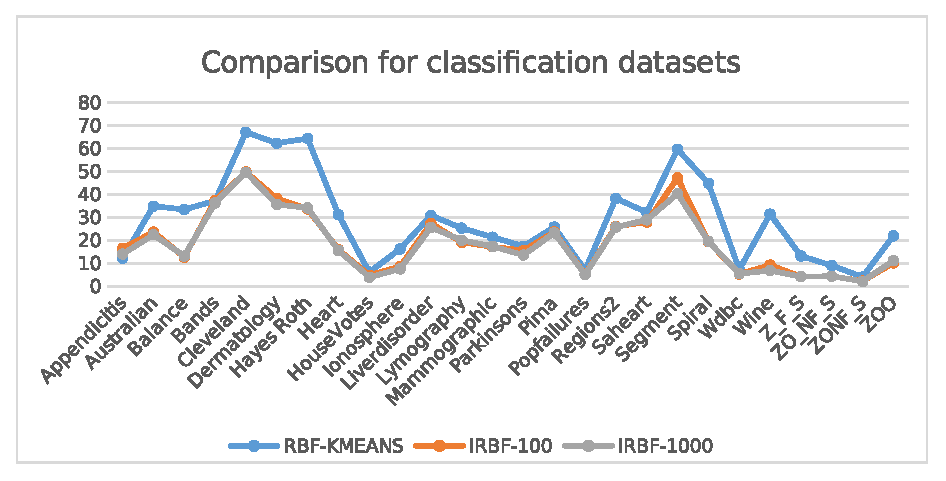
\includegraphics[scale=0.7]{classcomparison}
\end{figure}
\begin{figure}
\caption{Graphical comparison of the methods for the regression datasets.\label{fig:graph_regression}}

\begin{centering}
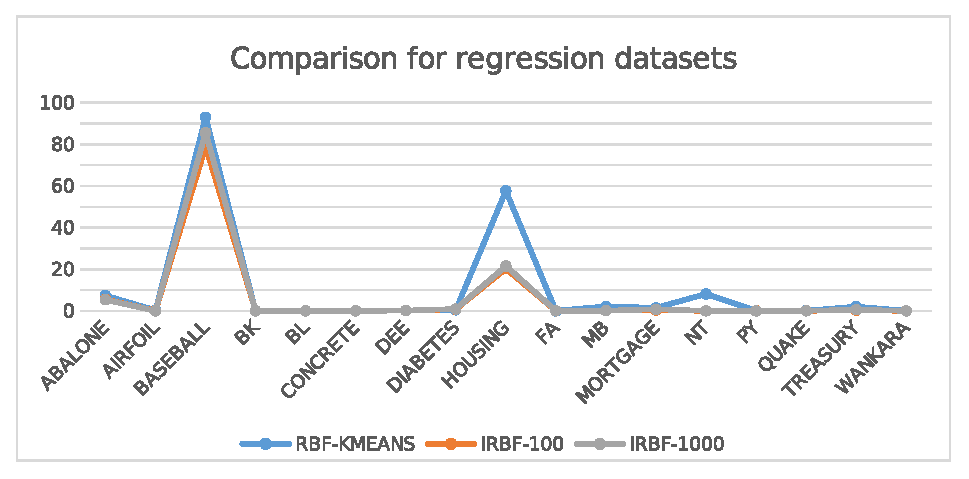
\includegraphics[scale=0.7]{regression_comparison}
\par\end{centering}
\end{figure}

\begin{table}
\caption{Experimental results using different values for the parameter $F$
on the classification datasets.\label{tab:expsFClass}}

\centering{}%
\begin{tabular}{|c|c|c|c|}
\hline 
DATASET & $F=3$ & $F=5$ & $F=10$\tabularnewline
\hline 
\hline 
Appendicitis & 14.43\% & 14.03\% & 14.47\%\tabularnewline
\hline 
Australian & 23.45\% & 22.39\% & 23.21\%\tabularnewline
\hline 
Balance & 13.35\% & 13.15\% & 11.79\%\tabularnewline
\hline 
Bands & 36.48\% & 36.29\% & 36.76\%\tabularnewline
\hline 
Cleveland & 49.26\% & 49.64\% & 49.02\%\tabularnewline
\hline 
Dermatology & 36.54\% & 35.64\% & 34.37\%\tabularnewline
\hline 
Hayes Roth & 39.28\% & 34.13\% & 36.46\%\tabularnewline
\hline 
Heart & 15.14\% & 15.60\% & 14.89\%\tabularnewline
\hline 
HouseVotes & 4.93\% & 3.90\% & 6.41\%\tabularnewline
\hline 
Ionosphere & 7.56\% & 7.52\% & 9.05\%\tabularnewline
\hline 
Liverdisorder & 28.37\% & 25.63\% & 28.97\%\tabularnewline
\hline 
Lymography & 20.12\% & 20.02\% & 21.05\%\tabularnewline
\hline 
Mammographic & 18.04\% & 17.30\% & 18.21\%\tabularnewline
\hline 
Parkinsons & 18.51\% & 13.59\% & 13.49\%\tabularnewline
\hline 
Pima & 23.69\% & 23.23\% & 23.52\%\tabularnewline
\hline 
Popfailures & 5.76\% & 5.10\% & 4.50\%\tabularnewline
\hline 
Regions2 & 25.79\% & 25.77\% & 25.32\%\tabularnewline
\hline 
Saheart & 28.89\% & 28.91\% & 26.99\%\tabularnewline
\hline 
Segment & 36.53\% & 40.28\% & 43.28\%\tabularnewline
\hline 
Spiral & 16.78\% & 19.56\% & 22.18\%\tabularnewline
\hline 
Wdbc & 4.64\% & 5.44\% & 5.10\%\tabularnewline
\hline 
Wine & 8.31\% & 6.84\% & 8.27\%\tabularnewline
\hline 
Z\_F\_S & 4.32\% & 4.18\% & 4.03\%\tabularnewline
\hline 
ZO\_NF\_S & 3.70\% & 4.35\% & 3.72\%\tabularnewline
\hline 
ZONF\_S & 2.04\% & 2.08\% & 1.98\%\tabularnewline
\hline 
ZOO & 11.87\% & 11.13\% & 9.97\%\tabularnewline
\hline 
\textbf{AVERAGE} & \textbf{18.65\%} & \textbf{18.68\%} & \textbf{19.12\%}\tabularnewline
\hline 
\end{tabular}
\end{table}
\begin{table}

\caption{Experimental results using different values for the parameter $F$
on the classification datasets.\label{tab:expsFRegression}}

\centering{}%
\begin{tabular}{|c|c|c|c|}
\hline 
DATASET & $F=3$ & $F=5$ & $F=10$\tabularnewline
\hline 
\hline 
ABALONE & 5.56 & 5.32 & 5.41\tabularnewline
\hline 
AIRFOIL & 0.004 & 0.003 & 0.004\tabularnewline
\hline 
BASEBALL & 88.40 & 85.58 & 84.43\tabularnewline
\hline 
BK & 0.03 & 0.03 & 0.02\tabularnewline
\hline 
BL & 0.0005 & 0.0003 & 0.0002\tabularnewline
\hline 
CONCRETE & 0.009 & 0.007 & 0.007\tabularnewline
\hline 
DEE & 0.18 & 0.16 & 0.16\tabularnewline
\hline 
DIABETES & 0.67 & 0.89 & 0.77\tabularnewline
\hline 
HOUSING & 20.03 & 21.54 & 20.84\tabularnewline
\hline 
FA & 0.03 & 0.029 & 0.036\tabularnewline
\hline 
MB & 0.19 & 0.09 & 0.26\tabularnewline
\hline 
MORTGAGE & 0.89 & 0.78 & 0.03\tabularnewline
\hline 
NT & 0.006 & 0.007 & 0.007\tabularnewline
\hline 
PY & 0.027 & 0.014 & 0.018\tabularnewline
\hline 
QUAKE & 0.04 & 0.03 & 0.04\tabularnewline
\hline 
TREASURY & 0.77 & 0.51 & 0.17\tabularnewline
\hline 
WANKARA & 0.002 & 0.002 & 0.002\tabularnewline
\hline 
\textbf{AVERAGE} & \textbf{6.87} & \textbf{6.76} & \textbf{6.60}\tabularnewline
\hline 
\end{tabular}
\end{table}


\section{Conclusions\label{sec:Conclusions}}

In this work, a two-stage technique for data classification and function
regression was presented using an RBF model. In the first stage of
the technique, an attempt is made to discover a promising range of
values for the network parameters and, in the second stage, the network
parameters are adjusted within this range using a genetic algorithm.
From the experiments performed, it appears that this technique is
in most cases much more efficient than the traditional training technique
of such models. Moreover, this technique appears to be largely robust,
as changes in its critical parameters do not entail large changes
in its reliability. However, the proposed technique is significantly
more time-consuming than the traditional training technique as it
requires computational time for both its phases. However, this problem
can be mitigated to a significant extent by the use of modern parallel
computing techniques.
\begin{thebibliography}{10}
\bibitem{physics_ml1}M. Mjahed, The use of clustering techniques
for the classification of high energy physics data, Nuclear Instruments
and Methods in Physics Research Section A: Accelerators, Spectrometers,
Detectors and Associated Equipment \textbf{559}, pp. 199-202, 2006.

\bibitem{physics_ml2}M Andrews, M Paulini, S Gleyzer, B Poczos, End-to-End
Event Classification of High-Energy Physics Data, Journal of Physics:
Conference Series \textbf{1085}, 2018.

\bibitem{chemistry_ml1}P. He, C.J. Xu, Y.Z. Liang, K.T. Fang, Improving
the classification accuracy in chemistry via boosting technique, Chemometrics
and Intelligent Laboratory Systems 70, pp. 39-46, 2004.

\bibitem{chemistry_ml2}J.A. Aguiar, M.L. Gong, T.Tasdizen, Crystallographic
prediction from diffraction and chemistry data for higher throughput
classification using machine learning, Computational Materials Science
\textbf{173}, 109409, 2020.

\bibitem{econ_ml1}I. Kaastra, M. Boyd, Designing a neural network
for forecasting financial and economic time series, Neurocomputing
\textbf{10}, pp. 215-236, 1996.

\bibitem{econ_ml2}R. Hafezi, J. Shahrabi, E. Hadavandi, A bat-neural
network multi-agent system (BNNMAS) for stock price prediction: Case
study of DAX stock price, Applied Soft Computing \textbf{29}, pp.
196-210, 2015.

\bibitem{med_ml1}S.S. Yadav, S.M. Jadhav, Deep convolutional neural
network based medical image classification for disease diagnosis.
J Big Data \textbf{6}, 113, 2019.

\bibitem{med_ml2}L. Qing, W. Linhong , D. Xuehai, A Novel Neural
Network-Based Method for Medical Text Classification, Future Internet
\textbf{11}, 255, 2019. 

\bibitem{rbf1}J. Park and I. W. Sandberg, Universal Approximation
Using Radial-Basis-Function Networks, Neural Computation \textbf{3},
pp. 246-257, 1991.

\bibitem{rbfghosh}J. Ghosh, A. Nag, An Overview of Radial Basis Function
Networks. In: Howlett, R.J., Jain, L.C. (eds) Radial Basis Function
Networks 2. Studies in Fuzziness and Soft Computing, vol 67. Physica,
Heidelberg, 2001.

\bibitem{rbfde1}Nam Mai-Duy, Thanh Tran-Cong, Numerical solution
of differential equations using multiquadric radial basis function
networks, Neural Networks 14, pp. 185-199, 2001.

\bibitem{rbfde2}N. Mai-Duy, Solving high order ordinary differential
equations with radial basis function networks. Int. J. Numer. Meth.
Engng. \textbf{62}, pp. 824-852, 2005.

\bibitem{rbfnetwork1}C. Laoudias, P. Kemppi and C. G. Panayiotou,
Localization Using Radial Basis Function Networks and Signal Strength
Fingerprints in WLAN, GLOBECOM 2009 - 2009 IEEE Global Telecommunications
Conference, Honolulu, HI, 2009, pp. 1-6, 2009.

\bibitem{rbfnetwork2}M. Azarbad, S. Hakimi, A. Ebrahimzadeh, Automatic
recognition of digital communication signal, International journal
of energy, information and communications \textbf{3}, pp. 21-33, 2012.

\bibitem{rbfphysics1}P. Teng, Machine-learning quantum mechanics:
Solving quantum mechanics problems using radial basis function networks,
Phys. Rev. E \textbf{98}, 033305, 2018.

\bibitem{rbfphysics2}R. Jovanovi\'{c}, A. Sretenovic, Ensemble of
radial basis neural networks with K-means clustering for heating energy
consumption prediction, FME Transactions \textbf{45}, pp. 51-57, 2017.

\bibitem{rbfchemistry1}D.L. Yu, J.B. Gomm, D. Williams, Sensor fault
diagnosis in a chemical process via RBF neural networks, Control Engineering
Practice \textbf{7}, pp. 49-55, 1999.

\bibitem{rbfchemistry2}V. Shankar, G.B. Wright, A.L. Fogelson, R.M.
Kirby, A radial basis function (RBF) finite difference method for
the simulation of reaction--diffusion equations on stationary platelets
within the augmented forcing method, Int. J. Numer. Meth. Fluids \textbf{75},
pp. 1-22, 2014.

\bibitem{rbfecon0}W. Shen, X. Guo, C. Wu, D. Wu, Forecasting stock
indices using radial basis function neural networks optimized by artificial
fish swarm algorithm, Knowledge-Based Systems 24, pp. 378-385, 2011.

\bibitem{rbfecon1}J. A. Momoh, S. S. Reddy, Combined Economic and
Emission Dispatch using Radial Basis Function, 2014 IEEE PES General
Meeting | Conference \& Exposition, National Harbor, MD, pp. 1-5,
2014.

\bibitem{rbfecon2}P. Sohrabi, B. Jodeiri Shokri, H. Dehghani, Predicting
coal price using time series methods and combination of radial basis
function (RBF) neural network with time series. Miner Econ 2021.

\bibitem{rbf_dos1}U. Ravale, N. Marathe, P. Padiya, Feature Selection
Based Hybrid Anomaly Intrusion Detection System Using K Means and
RBF Kernel Function, Procedia Computer Science \textbf{45}, pp. 428-435,
2015.

\bibitem{rbf_dos2}M. Lopez-Martin, A. Sanchez-Esguevillas, J. I.
Arribas, B. Carro, Network Intrusion Detection Based on Extended RBF
Neural Network With Offline Reinforcement Learning, IEEE Access \textbf{9},
pp. 153153-153170, 2021.

\bibitem{rbfadv}H. Yu, T. Xie, S. Paszczynski and B. M. Wilamowski,
Advantages of Radial Basis Function Networks for Dynamic System Design,IEEE
Transactions on Industrial Electronics v\textbf{ 58}, pp. 5438-5450,
2011.

\bibitem{rbfpar1}R. Yokota, L.A. Barba, M. G. Knepley, PetRBF ---
A parallel O(N) algorithm for radial basis function interpolation
with Gaussians, Computer Methods in Applied Mechanics and Engineering
\textbf{199}, pp. 1793-1804, 2010.

\bibitem{rbfpar2}C. Lu, N. Ma, Z. Wang, Fault detection for hydraulic
pump based on chaotic parallel RBF network, EURASIP J. Adv. Signal
Process. \textbf{2011}, 49, 2011.

\bibitem{rbfinit1}L.I. Kuncheva, Initializing of an RBF network by
a genetic algorithm, Neurocomputing \textbf{14}, pp. 273-288, 1997.

\bibitem{rbfinit2}F. Ros, M. Pintore, A. Deman, J.R. Chr�tien, Automatical
initialization of RBF neural networks, Chemometrics and Intelligent
Laboratory Systems \textbf{87}, pp. 26-32, 2007.

\bibitem{rbfinit3}D. Wang, X.J. Zeng, J.A. Keane, A clustering algorithm
for radial basis function neural network initialization, Neurocomputing
\textbf{77}, pp. 144-155, 2012.

\bibitem{rbfprun1}E. Ricci, R. Perfetti, Improved pruning strategy
for radial basis function networks with dynamic decay adjustment,
Neurocomputing \textbf{69}, pp. 1728-1732, 2006.

\bibitem{rbfprun3}Guang-Bin Huang, P. Saratchandran and N. Sundararajan,
A generalized growing and pruning RBF (GGAP-RBF) neural network for
function approximation, IEEE Transactions on Neural Networks \textbf{16},
pp. 57-67, 2005.

\bibitem{rbfprun2}M. Bortman and M. Aladjem, A Growing and Pruning
Method for Radial Basis Function Networks, IEEE Transactions on Neural
Networks \textbf{20}, pp. 1039-1045, 2009.

\bibitem{rbfcon1}N. B. Karayiannis, M. M. Randolph-Gips, On the construction
and training of reformulated radial basis function neural networks,
IEEE Transactions on Neural Networks \textbf{14}, pp. 835-846, 2003.

\bibitem{rbfcon2}J.X. Peng, K. Li, D.S. Huang, A Hybrid Forward Algorithm
for RBF Neural Network Construction, IEEE Transactions on Neural Networks,
\textbf{17}, pp. 1439-1451, 2006.

\bibitem{rbfcon3}D. Du, K. Li, M. Fei, A fast multi-output RBF neural
network construction method, Neurocomputing \textbf{73}, pp. 2196-2202,
2010.

\bibitem{kmeans}J. MacQueen, Some methods for classification and
analysis of multivariate observations, in: Proceedings of the fifth
Berkeley symposium on mathematical statistics and probability, Vol.
1, No. 14, pp. 281-297, 1967. 

\bibitem{interval0}E. Hansen and G.W. Walster.Global Optimization
using Interval Analy-sis.Marcel Dekker Inc., New York, 2004.

\bibitem{interval1}M.Cs. Mark�t,Fern�ndezL.G. and CasadoT. Csendes,
New interval methods for constrained global optimization, Mathematical
Programming \textbf{106}, pp. 287-318, 2006.

\bibitem{interval2}A. �ilinskas, and J. �ilinskas, Interval Arithmetic
Based Optimization in Nonlinear Regression, Informatica \textbf{21},
pp. 149-158, 2010.

\bibitem{interval_app1}C.A. Schnepper, M.A. Stadtherr, Robust process
simulation using interval methods, Computers \& Chemical Engineering
\textbf{20}, pp. 187-199, 1996.

\bibitem{interval_app2}C. Carreras, I. D. Walker, Interval methods
for fault-tree analysis in robotics, IEEE Transactions on Reliability
\textbf{50}, pp. 3-11, 2001.

\bibitem{interval_app3}A. Serguieva, J. Hunte, Fuzzy interval methods
in investment risk appraisal, Fuzzy Sets and Systems \textbf{142},
pp. 443-466, 2004.

\bibitem{pso1}Riccardo Poli, James Kennedy kennedy, Tim Blackwell,
Particle swarm optimization An Overview, Swarm Intelligence \textbf{1},
pp 33-57, 2007. 

\bibitem{kaelo}P. Kaelo, M.M. Ali, Integrated crossover rules in
real coded genetic algorithms, European Journal of Operational Research
\textbf{176}, pp. 60-76, 2007.

\bibitem{Tsoulos1}I.G. Tsoulos, Modifications of real code genetic
algorithm for global optimization, Applied Mathematics and Computation
\textbf{203}, pp. 598-607, 2008.

\bibitem{Keel}J. Alcal�-Fdez, A. Fernandez, J. Luengo, J. Derrac,
S. Garc�a, L. S�nchez, F. Herrera. KEEL Data-Mining Software Tool:
Data Set Repository, Integration of Algorithms and Experimental Analysis
Framework. Journal of Multiple-Valued Logic and Soft Computing 17,
pp. 255-287, 2011.

\bibitem{appendicitis}Weiss, Sholom M. and Kulikowski, Casimir A.,
Computer Systems That Learn: Classification and Prediction Methods
from Statistics, Neural Nets, Machine Learning, and Expert Systems,
Morgan Kaufmann Publishers Inc, 1991.

\bibitem{australian}J.R. Quinlan, Simplifying Decision Trees. International
Journal of Man-Machine Studies \textbf{27}, pp. 221-234, 1987. 

\bibitem{balance}T. Shultz, D. Mareschal, W. Schmidt, Modeling Cognitive
Development on Balance Scale Phenomena, Machine Learning \textbf{16},
pp. 59-88, 1994.

\bibitem{cleveland1}Z.H. Zhou,Y. Jiang, NeC4.5: neural ensemble based
C4.5,\textquotedbl{} in IEEE Transactions on Knowledge and Data Engineering
\textbf{16}, pp. 770-773, 2004.

\bibitem{cleveland2}R. Setiono , W.K. Leow, FERNN: An Algorithm for
Fast Extraction of Rules from Neural Networks, Applied Intelligence
\textbf{12}, pp. 15-25, 2000.

\bibitem{Bands}B. Evans, D. Fisher, Overcoming process delays with
decision tree induction, IEEE Expert \textbf{9}, pp. 60-66, 1994.

\bibitem{dermatology}G. Demiroz, H.A. Govenir, N. Ilter, Learning
Differential Diagnosis of Eryhemato-Squamous Diseases using Voting
Feature Intervals, Artificial Intelligence in Medicine. \textbf{13},
pp. 147--165, 1998.

\bibitem{hayesroth}B. Hayes-Roth, B., F. Hayes-Roth. Concept learning
and the recognition and classification of exemplars. Journal of Verbal
Learning and Verbal Behavior \textbf{16}, pp. 321-338, 1977.

\bibitem{heart}I. Kononenko, E. �imec, M. Robnik-�ikonja, Overcoming
the Myopia of Inductive Learning Algorithms with RELIEFF, Applied
Intelligence \textbf{7}, pp. 39--55, 1997

\bibitem{housevotes}R.M. French, N. Chater, Using noise to compute
error surfaces in connectionist networks: a novel means of reducing
catastrophic forgetting, Neural Comput. \textbf{14}, pp. 1755-1769,
2002.

\bibitem{ion1}J.G. Dy , C.E. Brodley, Feature Selection for Unsupervised
Learning, The Journal of Machine Learning Research \textbf{5}, pp
845--889, 2004.

\bibitem{ion2}S. J. Perantonis, V. Virvilis, Input Feature Extraction
for Multilayered Perceptrons Using Supervised Principal Component
Analysis, Neural Processing Letters \textbf{10}, pp 243--252, 1999.

\bibitem{liver} J. Garcke, M. Griebel, Classification with sparse
grids using simplicial basis functions, Intell. Data Anal. \textbf{6},
pp. 483-502, 2002.

\bibitem{lymography}G. Cestnik, I. Konenenko, I. Bratko, Assistant-86:
A Knowledge-Elicitation Tool for Sophisticated Users. In: Bratko,
I. and Lavrac, N., Eds., Progress in Machine Learning, Sigma Press,
Wilmslow, pp. 31-45, 1987. 

\bibitem{mammographic}M. Elter, R. Schulz-Wendtland, T. Wittenberg,
The prediction of breast cancer biopsy outcomes using two CAD approaches
that both emphasize an intelligible decision process, Med Phys. \textbf{34},
pp. 4164-72, 2007.

\bibitem{parkinsons}Little MA, McSharry PE, Hunter EJ, Spielman J,
Ramig LO. Suitability of dysphonia measurements for telemonitoring
of Parkinson's disease. IEEE Trans Biomed Eng. 2009;56(4):1015. doi:10.1109/TBME.2008.2005954

\bibitem{pima}J.W. Smith, J.E. Everhart, W.C. Dickson, W.C. Knowler,
R.S. Johannes, Using the ADAP learning algorithm to forecast the onset
of diabetes mellitus, In: Proceedings of the Symposium on Computer
Applications and Medical Care IEEE Computer Society Press, pp.261-265,
1988.

\bibitem{popfailures}D.D. Lucas, R. Klein, J. Tannahill, D. Ivanova,
S. Brandon, D. Domyancic, Y. Zhang, Failure analysis of parameter-induced
simulation crashes in climate models, Geoscientific Model Development
\textbf{6}, pp. 1157-1171, 2013.

\bibitem{regions}Giannakeas, N., Tsipouras, M.G., Tzallas, A.T.,
Kyriakidi, K., Tsianou, Z.E., Manousou, P., Hall, A., Karvounis, E.C.,
Tsianos, V., Tsianos, E. A clustering based method for collagen proportional
area extraction in liver biopsy images (2015) Proceedings of the Annual
International Conference of the IEEE Engineering in Medicine and Biology
Society, EMBS, 2015-November, art. no. 7319047, pp. 3097-3100. 

\bibitem{saheart}T. Hastie, R. Tibshirani, Non-parametric logistic
and proportional odds regression, JRSS-C (Applied Statistics) \textbf{36},
pp. 260--276, 1987.

\bibitem{segment}M. Dash, H. Liu, P. Scheuermann, K. L. Tan, Fast
hierarchical clustering and its validation, Data \& Knowledge Engineering
\textbf{44}, pp 109--138, 2003.

\bibitem{wdbc}W.H. Wolberg, O.L. Mangasarian, Multisurface method
of pattern separation for medical diagnosis applied to breast cytology,
Proc Natl Acad Sci U S A. \textbf{87}, pp. 9193--9196, 1990.

\bibitem{wine1}M. Raymer, T.E. Doom, L.A. Kuhn, W.F. Punch, Knowledge
discovery in medical and biological datasets using a hybrid Bayes
classifier/evolutionary algorithm. IEEE transactions on systems, man,
and cybernetics. Part B, Cybernetics : a publication of the IEEE Systems,
Man, and Cybernetics Society, \textbf{33} , pp. 802-813, 2003.

\bibitem{wine2}P. Zhong, M. Fukushima, Regularized nonsmooth Newton
method for multi-class support vector machines, Optimization Methods
and Software \textbf{22}, pp. 225-236, 2007.

\bibitem{eeg}R.G. Andrzejak, K. Lehnertz, F. Mormann, C. Rieke, P.
David, and C. E. Elger, Indications of nonlinear deterministic and
finite-dimensional structures in time series of brain electrical activity:
Dependence on recording region and brain state, Phys. Rev. E \textbf{64},
pp. 1-8, 2001.

\bibitem{zoo}M. Koivisto, K. Sood, Exact Bayesian Structure Discovery
in Bayesian Networks, The Journal of Machine Learning Research\textbf{
5}, pp. 549--573, 2004.

\bibitem{abalone}W. J Nash, T.L. Sellers, S.R. Talbot, A.J. Cawthor,
W.B. Ford, The Population Biology of Abalone (\_Haliotis\_ species)
in Tasmania. I. Blacklip Abalone (\_H. rubra\_) from the North Coast
and Islands of Bass Strait, Sea Fisheries Division, Technical Report
No. 48 (ISSN 1034-3288), 1994.

\bibitem{airfoil}T.F. Brooks, D.S. Pope, and A.M. Marcolini. Airfoil
self-noise and prediction. Technical report, NASA RP-1218, July 1989. 

\bibitem{Stat}J.S. Simonoff, Smooting Methods in Statistics, Springer
- Verlag, 1996.

\bibitem{concrete}I.Cheng Yeh, Modeling of strength of high performance
concrete using artificial neural networks, Cement and Concrete Research.
\textbf{28}, pp. 1797-1808, 1998. 

\bibitem{key23}D. Harrison and D.L. Rubinfeld, Hedonic prices and
the demand for clean ai, J. Environ. Economics \& Management \textbf{5},
pp. 81-102, 1978.

\bibitem{key21}J.S. Simonoff, Smooting Methods in Statistics, Springer
- Verlag, 1996.

\bibitem{ntdataset}Mackowiak, P.A., Wasserman, S.S., Levine, M.M.,
1992. A critical appraisal of 98.6 degrees f, the upper limit of the
normal body temperature, and other legacies of Carl Reinhold August
Wunderlich. J. Amer. Med. Assoc. 268, 1578--1580

\bibitem{pydataset}R.D. King, S. Muggleton, R. Lewis, M.J.E. Sternberg,
Proc. Nat. Acad. Sci. USA \textbf{89}, pp. 11322--11326, 1992. 

\bibitem{quake}M. Sikora, L. Wrobel, Application of rule induction
algorithms for analysis of data collected by seismic hazard monitoring
systems in coal mines, Archives of Mining Sciences \textbf{55}, pp.
91-114, 2010.

\bibitem{Armadillo}C. Sanderson, R. Curtin, Armadillo: a template-based
C++ library for linear algebra, Journal of Open Source Software \textbf{1},
pp. 26, 2016. 

\bibitem{openmp}R. Chandra, L. Dagum, D. Kohr, D. Maydan,J. McDonald
and R. Menon, Parallel Programming in OpenMP, Morgan Kaufmann Publishers
Inc., 2001.
\end{thebibliography}

\end{document}
